\documentclass[a4paper,chapter,atbegshi]{oblivoir}
\usepackage[dbl4x6]{fapapersize}
\usepackage{amsmath,amssymb,amsfonts,amsthm}
\usepackage{graphicx,xcolor,caption}
\usepackage{braket,hyperref,nicematrix}
\usepackage{euler,enumitem,tikz}
\usetikzlibrary{arrows.meta}
\setlist{nosep}
\hypersetup{
  colorlinks=true,linkcolor=teal,filecolor=magenta,urlcolor=cyan,
}
\title{\texttt{Introduction to Quantum Information Science} 학습일지}
\author{김태원}
\date{최초 작성 : 2023년 8월 29일 \\ 최근 편집 : \today}

\begin{document}
\maketitle
\break
\tableofcontents
\chapter{양자역학}
파인만{\tiny Richard Feynman}이 말하길 이중슬릿{\tiny double slit} 실험은
양자역학 전체를 요약한다. 

광자{\tiny photons}를 두 개의 슬릿{\tiny slit}을 지닌 벽에 하나씩 쏜다고 하자.
두 개의 슬릿 모두 개방될 때 광자가 특정 구간에 부딪히는 확률을 $P$, 1번 슬릿만
개방될 때 광자가 특정 구간에 부딪히는 확률을 $P_1$, 2번 슬릿만 개방될 때 광자가
특정 구간에 부딪히는 확률을 $P_2$라고 하자. 확률론에 따르면 당연히 $P=P_1+P_2$다.
그런데 실험 결과에 따르면 $P\neq P_1+P_2$다. 다시 말해 자연스러운 확률론은 자연의 
현상을 설명하지 못한다.

고전적인 확률론이 자연을 충분하게 설명하지 못하는데도 자연스러워 보이는 이유는 
\textbf{결어긋남\tiny decoherence}이라는 현상에서 비롯한다. 이를테면 상자를
열었을 때 슈뢰딩거의 고양이가 생과 사의 \emph{중첩\tiny superposition}으로
나타나지 않는다. 고양이가 제 환경과 끊임없이 상호작용하기 때문이다. 고양이와
환경 간의 상호작용은 고양이 계{\tiny system}의 정보를 누설한다. 반면 양자
중첩은 입자나 입자들의 군이 환경과 \emph{고립\tiny isolated}될 때 일어난다.

똑똑한 물리학자들이 이중슬릿 같은 실험을 통해 관찰한 바, 자연은 고전적인 확률
$P\in[0,1]$이 아니라 어떤 파동함수를 따른다. 그리고 이런 파동함수를 포착하는 
개념이 바로 \textbf{진폭\tiny amplitude} $\alpha\in\mathbb{C}$다. 양자역학에서
확률은 진폭을 사용해 \textbf{보른 규칙\tiny Born Rule}으로 정의된다. 보른 규칙은
보른{\tiny Max Born}이 양자계의 파동함수를 아우르는 슈뢰딩거 방정식의
해를 해석할 수 있는 유일한 방법으로 1926년에 제시한 공리다.
\begin{equation}\label{eq:11}
  P = |\alpha|^2 = \textrm{Real}(\alpha)^2+\textrm{Imaginary}(\alpha)^2
\end{equation}
진폭으로 이중슬릿 실험의 결과를 다시 확인하겠다. 두 슬릿 모두 개방될 때 광자가
특정 구간에 부딪히는 진폭을 $\alpha$, 1번 슬릿만 개방될 때 광자가 특정 구간에
부딪히는 진폭을 $\alpha_1$, 2번 슬릿만 개방될 때 광자가 특정 구간에
부딪히는 진폭을 $\alpha_2$라고 하자. 이떄 등식 $\alpha=\alpha_1+\alpha_2$는 모순을
유도하는가? $\alpha_1=a_1+b_1i, \alpha_2=a_2+b_2i$에 대해
\begin{align*}
  \alpha &= \alpha_1 + \alpha_2 \\
  \Rightarrow  P &= |\alpha|^2 \quad\quad\quad\quad[\textrm{보른 규칙}]\\ 
      &= |\alpha_1+\alpha_2|^2\\
      &= \textrm{Re}(\alpha_1+\alpha_2)^2+\textrm{Im}(\alpha_1+\alpha_2)^2\\
      &= (a_1+a_2)^2+(b_1+b_2)^2 \\
      &= (a_1^2+2a_1a_2+a_2^2)+(b_1^2+2b_1b_2+b_2^2) \\
      &= (a_1^2+b_1^2)+(a_2^2+b_2^2)+2(a_1a_2+b_1b_2)\\
      &= \textrm{Re}(\alpha_1)^2+\textrm{Im}(\alpha_1)^2+
      \textrm{Re}(\alpha_2)^2+\textrm{Im}(\alpha_2)^2+\overline{\alpha_1}\alpha_2+
      \alpha_1\overline{\alpha_2}\\
      &=|\alpha_1|^2+|\alpha_2|^2+\overline{\alpha_1}\alpha_2+
          \alpha_1\overline{\alpha_2} 
\end{align*}
이때 진폭이 복소수로 정의되기에 $\alpha$가 음수일 수 있으므로 모순이 유도되지
않는다는 사실을 아래처럼 나타낼 수 있다.
\[
  \alpha_1 := \frac{1}{2}, \alpha_2 := -\frac{1}{2} \Rightarrow
  \begin{cases}
    |\alpha_1|^2 = \frac{1}{4}, |\alpha_2|^2=\frac{1}{4} \\
              |\alpha=\alpha_1+\alpha_2|^2=0
  \end{cases}
\]
이처럼 두 상태의 진폭이 서로 소거할 수도 있다. \textbf{간섭\tiny
interference}이라는 현상이다. 간섭은 간단한 선형대수학으로 설명될 수 있다.
우선 2-노름{\tiny norm} $\alpha^2+\beta^2=1$을 충족하는 벡터 $(\alpha,\beta)$가
아래와 같은 원을 형성한다는 사실에 주목한다. 
\begin{figure}[h]
\begin{center}
  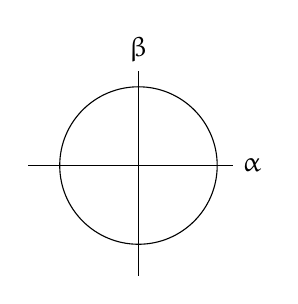
\begin{tikzpicture}
    \draw[fill=none](0,0)circle(1.0); 
    \draw[](0,-1.4)--(0,1.2) node[above]{$\beta$};
    \draw[](-1.4,0)--(1.2,0) node[right]{$\alpha$};
  \end{tikzpicture}
  \caption{유클리드 노름\label{fig:1-1}}
\end{center}
\end{figure}
2-노름을 유클리드 노름{\tiny Euclidean norm}이라고 부르기도 한다.
임의의 $\alpha,\beta$에 대해 위와 같은 원이 형성되기에 한 유클리드 노름 단위
벡터를 다른 유클리드 노름 단위 벡터로 사상하는{\tiny maps to} 행렬 혹은 변환이
존재할 수 있다. 이를 \textbf{유니타리 행렬\tiny unitary matrix}이라고 부른다.
또한 여기서 `유클리드 노름 단위 벡터'가 바로 \textbf{큐비트\tiny qubit}다. 

물리학자들은 디락{\tiny Paul Dirac}이 도입한 브라-켓{\tiny bra-ket} 표기법으로
큐비트를 나타낸다. 아래 같은 켓{\tiny ket} $\ket{\psi}$에 대해
 \[
   \ket{\psi} = \alpha\ket0+\beta\ket1 = \begin{pmatrix}\alpha\\\beta\end{pmatrix}
  =\alpha\begin{pmatrix}1\\0\end{pmatrix}+\beta\begin{pmatrix}0\\1\end{pmatrix} 
 \]
$\alpha$는 $\ket{0}$이라는 결과에 대한 진폭이고 $\beta$는 $\ket{1}$이라는
결과에 대한 진폭이다. 브라{\tiny bra} $\bra{\psi}$는 아래와 같다.
 \[
   \bra{\psi} = \overline{\alpha}\bra0 +\overline{\beta}\bra1=
   \begin{pmatrix}\overline{\alpha}&\overline{\beta}\end{pmatrix}
 \]
 이에 노름 $\|\psi\|^2$가 자연스럽게 정의될 수 있다. 
 \[
   \|\psi\|^2 = \begin{pmatrix}\overline{\alpha}&\overline{\beta}\end{pmatrix}
   \begin{pmatrix}\alpha\\\beta\end{pmatrix}=|\alpha|^2+|\beta|^2
 \]
 내적 $\braket{\psi|\phi}$는 아래 성질을 만족한다.
 \begin{align*}
   \braket{\psi|\phi} &= 
   \begin{pmatrix}\overline{\alpha_1} &\overline{\beta_1}\end{pmatrix}
   \begin{pmatrix}\alpha_2\\\beta_2\end{pmatrix} \\
    &= \overline{\alpha_1}\alpha_2+\overline{\beta_1}\beta_2\\
    &=\overline{\alpha_1}\overline{\overline{\alpha_2}}+
    \overline{\beta_1}\overline{\overline{\beta_2}} \\
    &= \begin{pmatrix}\overline{\overline{\alpha_2}} & \overline{\overline{\beta_2}}\end{pmatrix}
   \begin{pmatrix}\overline{\alpha_1}\\\overline{\beta_2}\end{pmatrix}
   = \overline{\braket{\phi|\psi}}
 \end{align*}
이에 행렬을 $45^{\circ}$ 즉 $\frac{\pi}{4}$만큼 회전하며 노름을 보존하는
아래 같은 유니타리 행렬이 있다.
\[
  \begin{pmatrix}
    \cos\frac{\pi}{4} &-\sin\frac{\pi}{4}\\
    \sin\frac{\pi}{4} &\cos\frac{\pi}{4}
  \end{pmatrix}
  = \begin{pmatrix}
    \frac{1}{\sqrt{2}} &-\frac{1}{\sqrt{2}} \\
    \frac{1}{\sqrt{2}} &\frac{1}{\sqrt2}
  \end{pmatrix}
\]
$\ket0$를 위 유니타리 행렬로 변환한다.
\begin{equation}\label{eq:1-2}
  \begin{pmatrix}
    \frac{1}{\sqrt{2}} &-\frac{1}{\sqrt{2}} \\
    \frac{1}{\sqrt{2}} &\frac{1}{\sqrt2}
  \end{pmatrix}
  \begin{pmatrix}
    1\\0
  \end{pmatrix}
  =\begin{pmatrix}
    \frac{1}{\sqrt2}\\\frac{1}{\sqrt2}
  \end{pmatrix}
\end{equation}
$\frac{1}{\sqrt2}\ket{0}+\frac{1}{\sqrt2}\ket{1}$을 다시 위 유니타리 행렬로
변환한다.
\[
  \begin{pmatrix}
    \frac{1}{\sqrt{2}} &-\frac{1}{\sqrt{2}} \\
    \frac{1}{\sqrt{2}} &\frac{1}{\sqrt2}
  \end{pmatrix}
  \begin{pmatrix}
    \frac{1}{\sqrt2}\\\frac{1}{\sqrt2}
  \end{pmatrix}
  =\begin{pmatrix}0\\1\end{pmatrix}=\ket{1}
\]
즉 무작위 상태 $\frac{1}{\sqrt2}\ket{0}+\frac{1}{\sqrt2}\ket{1}$에 위 유니타리
행렬과 같은 무작위 연산을 적용하면 $\ket{1}$이라는 결과가 결정론적{\tiny
deterministic}으로 나온다. 여기 무작위 연산을 다시 적용하여 나타난 무작위 상태
 $-\frac{1}{\sqrt2}\ket{0}+\frac{1}{\sqrt2}\ket{1}$에 무작위 연산을 또다시
 적용하면 $\ket{0}$이라는 결과가 결정론적으로 나온다. 이것이 앞서 언급한
 \textbf{간섭} 개념의 선형대수학적 바탕이다. 

 위 유니타리 행렬에 대해 $\ket{0}$이라는 결과를 결정론적으로 도출하는 행렬은
 $\frac{1}{\sqrt2}\ket0-\frac{1}{\sqrt2}\ket{1}$이다. 이를 \textbf{경로\tiny
 path}가 두 개 존재하여 한 경로는 음의 진폭 $-\frac{1}{\sqrt2}$를 지니고 
 다른 경로는 양의 진폭 $\frac{1}{\sqrt2}$을 지닌다고 표현한다. 그리고 이 경우
 두 경로는 \textbf{파괴적 간섭\tiny destructive interference} 관계에 놓인다. 
 반면 $\ket{1}$이라는 결과를 결정론적으로 도출하는 경로는 모두 양의 진폭
 $\frac{1}{\sqrt2}$을 지녀 \textbf{구성적 간섭\tiny constructive interference}
 관계다.

 이제 그림 \ref{fig:1-1}상의 원을 다시 그린다.
\begin{figure}[h]
\begin{center}
  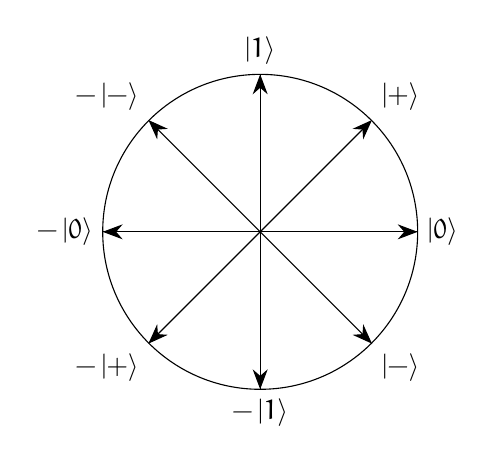
\begin{tikzpicture}
    \draw[fill=none](0,0)circle(2.0);
    \draw[-{Stealth[scale=1.5]}] (0,0)--(0,2);
    \draw[-{Stealth[scale=1.5]}] (0,0)--(-2,0) node[left]{$-\ket0$};
    \draw[-{Stealth[scale=1.5]}] (0,0)--(1.42,1.42) node[above right]{$\ket+$};
    \draw[-{Stealth[scale=1.5]}] (0,0)--(2,0);
    \draw[-{Stealth[scale=1.5]}] (0,0)--(-1.42,1.42) node[above left]{$-\ket-$};
    \draw[-{Stealth[scale=1.5]}] (0,0)--(1.42,-1.42) node[below right]{$\ket-$};
    \draw[-{Stealth[scale=1.5]}] (0,0)--(0,-2) node[below]{$-\ket1$};
    \draw[-{Stealth[scale=1.5]}] (0,0)--(-1.42,-1.42) node[below left]{$-\ket+$};
    \draw[](0,-2.0)--(0,2.0) node[above]{$\ket1$};
    \draw[](-2.0,0)--(2.0,0) node[right]{$\ket0$};
  \end{tikzpicture}
  \caption{직교 행렬\label{fig:1-2}}
\end{center}
\end{figure}
$\{\ket+,\ket-\}$는 \emph{아다마르 기저\tiny Hadamard basis}라고 부르는데
앞서 예로 든 $45^{\circ}$ 회전 유니타리 변환 과정 \ref{eq:1-2}에서 이미
확인한 것들이다. 
\[
  \begin{pmatrix}\frac{1}{\sqrt2}\\\frac{1}{\sqrt2}\end{pmatrix}=\ket+ =
  \frac{\ket0+\ket1}{\sqrt2},\quad\begin{pmatrix}\frac{1}{\sqrt2}\\
  -\frac{1}{\sqrt2}\end{pmatrix} = \ket-=\frac{\ket0-\ket1}{\sqrt2}
\]
그림 \ref{fig:1-2}에서 확인할 수 있는 사실은 $\frac{\pi}{4}$
회전과 반사만으로 여덟 가지 상태를 나타낼 수 있다는 것이다. 이는
\textbf{직교행렬}{\tiny ortoogonal matrix}이 지니는 성질이다. 
이외에도 대표적인 유니타리 행렬로는 아래 같은 것들이 있다.
\[\begin{matrix}
  \textrm{ 항등변환 }&\begin{pmatrix}1 & 0 \\ 0 & 1\end{pmatrix} 
  \textrm{ NOT게이트 }&\begin{pmatrix}0 & 1 \\ 1 & 0\end{pmatrix} \\
  \textrm{ 상대위상조정}&\begin{pmatrix}1&0\\0&i\end{pmatrix}
  \textrm{ 2차원 회전 }&\begin{pmatrix}\cos\theta & -\sin\theta\\
  \sin\theta &\cos\theta\end{pmatrix}
  \end{matrix}\]
또한 그림 \ref{fig:1-2}상의 원은 유클리드 노름을 보존한다. 따라서
임의의 유니타리 행렬 $U$의 복소전치행렬 $U^{\dagger}$에 $U$로 변환하면
항등행렬 $I$가 나온다.
\[
  \braket{\psi|\psi} = (\ket{\psi})^{\dagger}\ket{\psi} 
              = (U\ket{\psi})^{\dagger}U\ket{\psi}
              =\braket{\psi|U^{\dagger}U|\psi} 
  \iff\forall\ket{\psi},U^{\dagger}U= I
\]
유니타리 변환은 결국 선형변환이다. 그래서 $U(c\ket0)=cU\ket0$이 임의의 상수 $c$에 
대해 성립할 수 있다. 여기서 $c$가 어떤 $\theta$에 대해 오일러 공식 
$e^{i\theta}=\cos\theta+i\sin\theta$\footnote{오일러 공식은 슈뢰딩거
방정식을 비롯해 양자역학에서 중요한 파동-삼각함수를 지수함수로 변환할 수 있도록
하는, 복소평면에서 일정한 속도로 원운동하는 물체의 위치 방정식이다.}를 만족하면 
\textbf{전역위상\tiny global phase}이라고 한다. 요점은 $\ket{\psi}$와 
$e^{i\theta}\ket{\psi}$가 물리적으로 구분될 수 없으므로 전역위상이
관찰불가능하다는 것이다. 전역위상이 관찰가능하다는 말은 큐비트와 같은
양자계에 어떤 스칼라를 곱해서 우주 전체를 살짝 옮길 수 있다는
소리와 같다.

이에 반해 관찰 가능한 것은 바로 \textbf{상대위상\tiny relative
phase}이다. 이를테면 $\ket+$와 $\ket-$라는 두 상태 간에는 상대위상차이가 관측될
수 있다. $\ket-$에서 $\ket+$에 이르는 일련의 유니타리 연산들이 존재하기 때문이다.
\end{document}
